%
% Latex template for term paper in PHY 493
% Author: Jason Gombas
% Date: Feb 2021
%
% Modifications:
% Mar 2021, Reinhard Schwienhorst, update to make it generic and to use bibtex
%
% Usage instructions:
% This template uses revtex4 from the APS, see https://journals.aps.org/revtex
% This example uses revtex4-1, but it also works with revtex4-2
% This is commonly available in most latex distributions, or you can download it
% Use bibtex for the bibliography, the file "main.bib" is the input file to which you should add your 
% citations.
% To compile: run pdflatex and bibtex
%  pdflatex main; pdflatex main; bibtex main; pdflatex main 
% The output will be file main.pdf. 
%
\RequirePackage{lineno} % the lineno package provides line numbering, very helpful for reviewing the paper
\documentclass[amsfonts, amssymb, amsmath, preprint, showkeys, nofootinbib,longbibliography]{revtex4-1}
\usepackage{graphicx} % for figures
\usepackage[english]{babel}  % spelling
\usepackage[utf8]{inputenc}
\usepackage[pdftex, pdftitle={Article}, pdfauthor={Author}]{hyperref} % For hyperlinks in the PDF
%\setlength{\marginparwidth}{2.5cm}


\begin{document}
\linenumbers

\title{\Large My title}

\author{Author Name}

\date{\today} % Leave empty to omit a date

\begin{abstract} \normalsize
My abstract, a brief summary of the paper. 

\end{abstract}

\maketitle

\section{Introduction}

\begin{figure}[h]
	\centering
	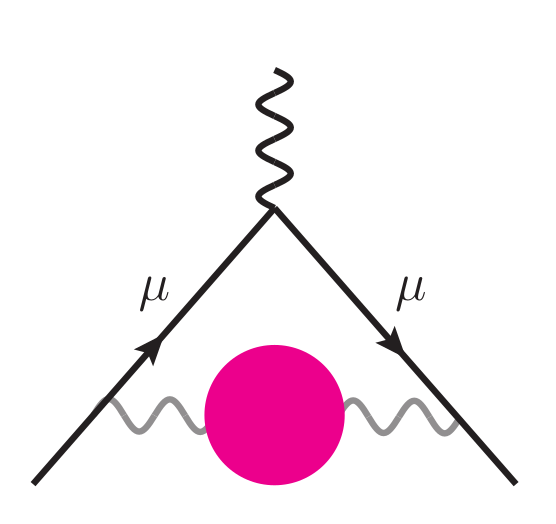
\includegraphics[width=0.45\linewidth]{figures/paperFig1.png}
	\caption{%
		Figure 1 from \cite{Davies_2020}.
	}
	\label{fig: paperFig1}
\end{figure}

The objective of this paper is to calculate the contribution of the muon anomalous magnetic moment hadronic vacuum polarization from the connected diagrams of up and down quarks, omitting electromagnetism.
In order to do this, It employs QCD guage-field configurations with dynamical $u,d,s,$ and $c$ quarks and the physical pion mass, and analyze five ensembles with different lattice spacings ($a \approx 0.06$fm to $a \approx 0.15$fm).

\section{Background and Methodology}
The relation between the leading-order hadronic-vacuum-polarization contribution to the muon’s anomalous magnetic moment and the renormalized quark vacuum polarization function $\hat{\Pi}(Q^2) \equiv \Pi(Q^2) - \Pi(0)$, is given by
\begin{equation}
	a_\mu^{HVP,LO} = \left(\frac{\alpha}{2}\right)^2 \int_0^\infty \dd{Q^2} K_E (Q^2) \hat{\Pi}(Q^2).
\end{equation}
\begin{equation}
	G(t) = \frac{1}{27} \int \dd{\vb{x}} \left[4\ev{j_i^u(\vb{x},t)j_i^u(0,0)} + \ev{j_i^d(\vb{x},t),j_i^d(0,0)}\right].
\end{equation}
\begin{equation}
	\hat{\Pi}(\omega^2) = \frac{4\pi^2}{\omega^2} \int_0^\infty \dd{t} G(t) \left[\omega^2t^2-4\sin[2](\frac{\omega t}{2})\right].
\end{equation}
\begin{equation}
	\hat{\Pi}(Q^2) = \frac{Q^2}{3} \int_0^\infty \dd{s}\frac{R_\gamma(s)}{s(s+Q^2)},
\end{equation}
where
\begin{equation}
	R_\gamma (s) \equiv \frac{\sigma(e^+e^- \rightarrow \gamma^* \rightarrow \text{hadrons})}{4\pi\alpha(s)^2/(3s)}.
\end{equation}

\section{Lattice-QCD Calculation}
\label{sec: LatCalc}

\begin{table*}[!b]
	% \centering
	\noindent\makebox[\linewidth]{%
	$
	\begin{array}{ccccccccc}
		\hline\hline
		\approx a \text{(fm)}
		& am_l^{\text{sea}}/am_s^{\text{sea}}/am_c^{\text{sea}}
		& w_0/a
		& Z_{V,\bar{s}s}
		& M_{\pi_5} \text{(MeV)}
		& E_{2\pi,\text{min}}\text{(MeV)}
		& (L/a)^3\times(T/a)
		& N_{\text{conf.}}
		& N_{\text{wall}}
		\\\hline
		0.15 & 0.00235/0.0647/0.831 & 1.13670(50) & 0.9881(10) & 133.04(70) & 640.4(3.4) & 32^3\times 48 & 997
		& 16\\
		0.15 & 0.002426/0.0673/0.8447 & 1.13215(35) & 0.9881(10) & 134.73(71) & 639.7(3.4) & 32^3 \times 48 & 9362 & 48 \text{(TSM)}\\
		0.12 & 0.00184/0.0507/0.628 & 1.41490(60) & 0.99220(40) & 132.73(70) & 540.8(3.3) & 48^3 \times 64 & 998 & 16\\
		0.09 & 0.00120/0.0363/0.432 & 1.95180(70) & 0.99400(50) & 128.34(68) & 524.3(2.8) & 64^3 \times 96 & 1557 & 16 \text{(TSM)}\\
		0.06 & 0.0008/0.022/0.260 & 3.0170(23) & 0.9941(11) & 134.95(72) & 530.8(2.8) & 96^3 \times 192 & 1230 & 16 \text{(TSM)}
		\\\hline\hline
	\end{array}
	$
	}
	\caption{%
	"Table I" from \cite{Davies_2020}.
	}
	\label{tab: 1}
\end{table*}

% In this section, they first present the lattice quark and gluon actions employed and the parameters of the QCD gauge-field configurations and correlation functions.
% Next, in section \ref{sec: LatCalc}\ref{sec: LatCalcB}, extract $a_\mu^{ud}$(conn.) in the isospin-symmetric limit on each ensemble from the vector-current correlation functions.
% Last, in section \ref{sec: LatCalc}\ref{sec: LatCalcC}, we correct the results for the isospin-symmetric $a_\mu^{ud}$(conn.) on each ensemble for finite-volume and taste-breaking discretization errors, and subsequently extrapolate these corrected values to zero lattice spacing.


\subsection{Numerical Simulation}
\label{sec: LatCalcA}
They perform their calculation on QCD gauge-field configurations generated by the MILC Collaboration with four flavors of HISQ quarks.
These configurations are isospin-symmetric, i.e., the up and down sea-quark masses are equal with a mass $ m_l = (m_u + m_d)/2 $.

Two of the ensembles listed in table \ref{tab: 1} were also used in \cite{PhysRevD.96.034516}:
the $a \approx 0.15$fm ensemble with approximately 1000 configurations and the $a \approx 0.12$fm ensemble.
In addition, a new ensemble is included with $a \approx 0.15$fm and parameters identical to the older $a \approx 0.15$fm physical-mass ensemble, except for having better tuned quark masses.
Thus, comparing this high-statistics ensemble and the older low-statistics one enables us to test our methods for extracting all $ a_\mu^{ll}$(conn.) from noisy data.

On the three newer ensembles analyzed in this work, they employ in addition a cost-effective variance-reduction technique called the truncated solver method (TSM).
With this approach, on each configuration they compute a large number of “sloppy” correlators with a large relative error of $10^{−5}$ at a small cost, and a single “fine” correlator with a small relative error of $10^{−8}$.
The use of the TSM reduces computational costs by a factor of $>2$.


\subsection{Extraction of Muon Anomaly}
\label{sec: LatCalcB}
\begin{figure}[h]
	\centering
	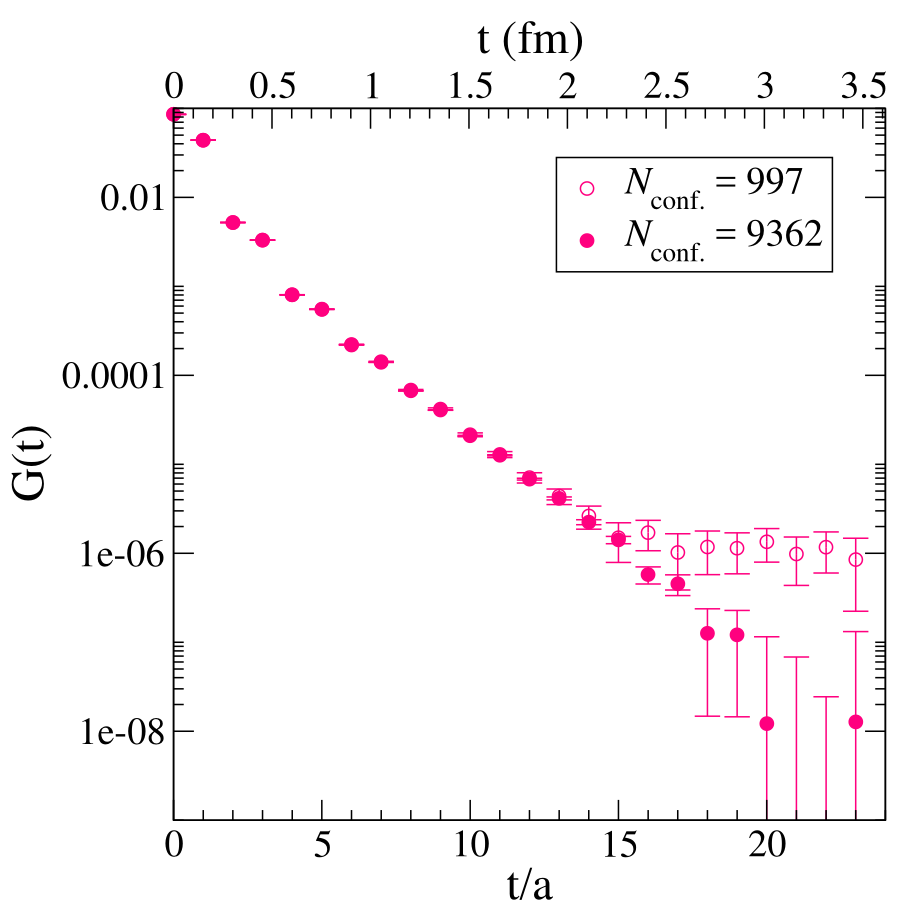
\includegraphics[width=0.45\linewidth]{figures/paperFig2.png}
	\caption{%
	Figure 2 from \cite{Davies_2020}.
	}
	\label{fig: paperFig2}
\end{figure}

A challenge common to all lattice-QCD calculations
of $a_\mu^{ll}$ (conn.) is the large statistical noise in the vector- current correlator at the physical light-quark mass.
Figure \ref{fig: paperFig2} shows the local-local vector-current correlator $G(t)$ on the two $a \approx 0.15$fm ensembles.
The correlator values at times $t$ and $T-t$ are averaged to increase statistics.
Beyond this range, the data with low statistics become too noisy to yield a reliable estimate of the correlation function.
Several strategies to address the noise problem can used.
In this paper, the same strategy is used as in \cite{PhysRevD.96.034516}.

\subsection{Lattice Corrections and Continuum Extrapolation}
\label{sec: LatCalcC}

Before extrapolating the values obtained for $a_\mu^{ll}$(conn.) in the previous section to zero lattice spacing, The data are corrected for the finite lattice spatial volume and for dis cretization effects from the mass splittings between staggered pions of different tastes.
Both effects arise from one-loop diagrams with $\pi\pi$ intermediate states.

For staggered quarks, the sea-pion masses are heavier than the taste-Goldstone pion for other representations of the approximate SO(4) taste symmetry.
Consequently, the combined finite-volume plus discretization corrections are largest for the coarsest lattices, and decrease toward the continuum.

One can test the estimates of the lattice corrections by comparing our results for the Taylor coefficients of the vacuum-polarization function with phenomenological determinations from R-ratio data.
Because the experimental data include all possible diagrammatic contributions, for this test, they use the full one-loop correction, which includes both the connected and disconnected pieces.

\section{Results}
In this section, the results for $a_\mu^{ll}\text{(conn.)}, \Pi_1^{ll} , \Pi_2^{ll} ,$ and $a_\mu^{\text{HVP,LO}}$ and the slope and curvature of $\hat{\Pi}(Q^2)$ comprehensive error budgets are presented.

\subsection{Light-Quark Connected Contribution}

Their numerical calculation of $a_\mu^{ll}$(conn.) and the slope and curvature of the renormalized vacuum-polarization function is with equal up- and down-quark masses, and without electromagnetism.
The results in the isospin-symmetric limit are
\begin{align}
	a_\mu^{ll} \text{(conn.)} &= 637.8(8.8) \times 10^{-10},\label{eq: a rez}\\
	\Pi_1^{ll} \text{(conn.)} &= 0.0932(14) \text{GeV}^2,\\
	\Pi_2^{ll} \text{(conn.)} &= -0.2089(64) \text{GeV}^4.
\end{align}

They obtained a total uncertainty of $1.4\%$ on the light-quark connected contribution to $a_\mu^{\text{HVP,LO}}$ in the isospin-symmetric limit without electromagnetism.

\subsection{Isospin-Breaking, Electromagnetic, and Quark-Disconnected Contributions}
To be able to compare the total summed over all quark flavors with experiment, one needs to correct the result for $a_\mu^{ll}$(conn.) (equation \ref{eq: a rez})

\subsubsection{$\pi\pi$ Corrections}
A large part of the isospin, electromagnetic, and quark-disconnected corrections comes from diagrams in figure \ref{fig: paperFig1} with $\pi\pi$ intermediate states.
These corrections can be estimated using the leading term in the chiral model.

They arrived at a total $\pi\pi$ correction to $a_\mu^{\text{HVP,LO}}$ from strong-isospin breaking, electromagnetism, and quark-disconnected diagrams of
\begin{equation}
	\Delta a_\mu^{\pi\pi}\text{(disc.)} = -12(3) \times 10^{-10}.
	\label{eq: pipi}
\end{equation}

\subsubsection{Residual Light-Quark Disconnect Corrections}

There are also quark-line disconnected corrections to $a_\mu^{\text{HVP,LO}}$ that have nothing to do with the $\pi\pi$ contribution.
One can estimate these by examining the contributions to the anomaly from the $\rho$ and $\omega$ mesons.
These resonances, together, account for almost $80\%$ of the total $a_\mu^{\text{HVP,LO}}$.
They retrieve a disconnected contribution from non-$\pi\pi$ states of
\begin{equation}
	\Delta a_\mu^{\rho\omega} \text{(disc.)} = -5(5)\times 10^{-10}.
	\label{eq: rhoomega}
\end{equation}

\subsubsection{Residual Strong-Isospin Breaking Corrections}

The effects from QCD-isospin breaking (i.e., quark-mass differences) and QED are intertwined both in nature and in lattice-QCD simulations.
In the paper, they define the residual strong-isospin correctioon to $a_\mu^{\text{HVP,LO}}$ as the shift relative to the isospin-symmetric value $a_\mu^{ll}$(conn.) that results when the bare $u$ and $d$ quark masses are retuned separately.
They found a relative correction of $\delta a_\mu^{\text{HVP,LO}}\text{(SIB)} = 1.5(7)\%$, which translates to an absolute correction of $\Delta a_\mu^{\text{HVP,LO}}\text{(SIB)}=9.5(4.5) \times 10^{-10}$, when commined with $a_\mu^{ll}$(conn.) from \ref{eq: a rez}.
They conclude by increasing the errors on their initial estimate of the total residual correction from strong-isospin breaking to allow for disconnected contributions of a commensurate size, giving
\begin{equation}
	\Delta a_\mu^{ud} \text{(SIB)} = 10(10) \times 10^{-10}.
	\label{eq: ud SIB}
\end{equation}


\subsubsection{Residual QED Corrections}
They estimate the residual corrections from QED, beyond those accounted for above, via power-counting to be of order $α \sim 1\%$.
This yields an estimate for the absolute correction to $a_\mu^{\text{HVP,LO}}$ of
\begin{equation}
	\Delta a_\mu^{ud}\text{(QED)} = 0(5) \times 10^{-10}.
	\label{eq: ud QED}
\end{equation}

\subsubsection{Total Contribution from $u/d$ Quarks}

Summing the corrections from equations \ref{eq: pipi} and equations \ref{eq: rhoomega}-\ref{eq: ud QED} gives the total correction from strong-isospin breaking, QED, and quark-disconnectedcontributions:
\begin{equation}
	\Delta a_\mu^{ud} \text{(SIB,QED,disc.)} = -7(13)\times 10^{-10}.
\end{equation}
Adding this to $a_\mu^{ll}$(conn.) (equation \ref{eq: a rez}) gives the total contribution to $a_\mu^{HVP,LO}$ from light quarks:
\begin{equation}
	a_\mu^{ud} = 630.8(8.8)(13) \times 10^{-10},
	\label{eq: a ud TOT}
\end{equation}
where the first error is from $a_\mu^{ll}$(conn.) and the second error is from $\Delta a_\mu^{ud}$.

\subsection{Total Leading-Order Contribution}

Finally, to obtain the total leading-order hadronic vacuum polarization contribution to $a_\mu$, they add the contributions from heavy flavors to $a_\mu^{ud}$ (equation \ref{eq: a ud TOT}):
\begin{equation}
	a_\mu^{\text{HVP,LO}} = 699(15)_{u,d} (1)_{s,c,b} \times 10^{-10}.
\end{equation}
Disconnected contributions from these quarks are expected to be negligible compared with our other uncertainties.

\clearpage

\bibliography{main}

\end{document}
